\documentclass[a4paper,11pt,oneside]{report}
\usepackage[margin=21mm,top=20mm,bottom=21mm,headheight=15pt,headsep=7mm]{geometry}
\usepackage{fontspec,microtype,graphicx,xcolor,tikz,titlesec,fancyhdr,enumitem,booktabs,tabularx,listings,hyperref,xurl,caption}
\usetikzlibrary{positioning,arrows.meta,calc,fit,shapes.geometric}
\setmainfont{Liberation Serif}
\setsansfont{Liberation Sans}
\setmonofont{DejaVu Sans Mono}[Scale=0.79]
\definecolor{ink}{HTML}{182735}
\definecolor{teal}{HTML}{087F8C}
\definecolor{pale}{HTML}{EDF5F6}
\definecolor{muted}{HTML}{526472}
\definecolor{amber}{HTML}{9C5C13}
\hypersetup{colorlinks=true,linkcolor=teal,urlcolor=teal,citecolor=teal,pdftitle={Meta-Harness: Architecture, Engineering, and User Guide},pdfauthor={Meta-Harness Project},pdfsubject={Implementation-based technical manual, October 2026}}
\setlength{\parindent}{0pt}
\setlength{\parskip}{6pt}
\setlength{\emergencystretch}{3em}
\raggedbottom
\setlist{nosep,leftmargin=*,topsep=4pt,itemsep=3pt}
\setlist[description]{style=nextline,leftmargin=0pt,labelindent=0pt}
\setcounter{tocdepth}{0}
\titleformat{\chapter}[display]{\sffamily\bfseries\color{ink}\LARGE}{\sffamily\small\color{teal}CHAPTER \thechapter}{2mm}{}
\titlespacing*{\chapter}{0pt}{-5pt}{9pt}
\titleformat{\section}{\sffamily\bfseries\large\color{ink}}{\thesection}{.6em}{}
\titlespacing*{\section}{0pt}{10pt}{4pt}
\titleformat{\subsection}{\sffamily\bfseries\normalsize\color{teal}}{\thesubsection}{.6em}{}
\titlespacing*{\subsection}{0pt}{8pt}{3pt}
\pagestyle{fancy}\fancyhf{}
\fancyhead[L]{\sffamily\small\bfseries META-HARNESS}
\fancyhead[R]{\sffamily\scriptsize\color{muted}\leftmark}
\fancyfoot[L]{\sffamily\scriptsize\color{muted}Engineering manual \;|\; 9 October 2026}
\fancyfoot[R]{\sffamily\scriptsize\thepage\ /\ \pageref{manualend}}
\renewcommand{\headrulewidth}{.4pt}
\renewcommand{\chaptermark}[1]{\markboth{\thechapter\quad #1}{}}
\fancypagestyle{plain}{\fancyhf{}\fancyhead[L]{\sffamily\small\bfseries META-HARNESS}\fancyhead[R]{\sffamily\scriptsize\color{muted}\leftmark}\fancyfoot[L]{\sffamily\scriptsize\color{muted}Engineering manual \;|\; 9 October 2026}\fancyfoot[R]{\sffamily\scriptsize\thepage\ /\ \pageref{manualend}}}
\newcommand{\partlabel}[1]{{\sffamily\small\color{teal}\textbf{#1}}\par\medskip}
\newcommand{\status}[1]{{\sffamily\small\textbf{\color{teal}#1}}}
\newcommand{\source}[1]{\par\medskip\begingroup\setlength{\fboxsep}{7pt}\noindent\colorbox{pale}{\begin{minipage}{\dimexpr\linewidth-14pt}\footnotesize\raggedright\sffamily\textbf{Source map}\quad #1\end{minipage}}\endgroup\par}
\newcommand{\note}[2]{\par\medskip{\sffamily\bfseries\color{teal}#1}\par #2\par}
\newcommand{\nextpage}[1]{\clearpage\section*{#1}}
\newcommand{\screenshot}[3]{\begin{center}\includegraphics[width=#2\linewidth]{figures/#1}\captionof{figure}{#3}\end{center}}
\captionsetup{font=small,labelfont={sf,bf},textfont=sf,skip=5pt,hypcap=false}
\lstset{basicstyle=\ttfamily\footnotesize,backgroundcolor=\color{pale},frame=none,breaklines=true,columns=fullflexible,keepspaces=true,showstringspaces=false,xleftmargin=6pt,xrightmargin=6pt,aboveskip=6pt,belowskip=6pt}
\tikzset{box/.style={draw=teal!65,rounded corners=2pt,fill=pale,align=center,font=\sffamily\small,text width=3.1cm,minimum height=1cm,inner sep=5pt},darkbox/.style={box,fill=ink,text=white,draw=ink},decision/.style={diamond,aspect=2.3,draw=teal,fill=pale,align=center,font=\sffamily\small,inner sep=2pt},arr/.style={-{Stealth[length=2mm]},draw=muted,thick},lab/.style={font=\sffamily\scriptsize,fill=white,inner sep=2pt}}
\begin{document}
\begin{titlepage}
\thispagestyle{empty}
\begin{tikzpicture}[remember picture,overlay]
\fill[ink] (current page.north west) rectangle ([yshift=-76mm]current page.north east);
\fill[teal] ([yshift=-76mm]current page.north west) rectangle ([yshift=-79mm]current page.north east);
\end{tikzpicture}
\vspace*{11mm}
{\sffamily\color{white}\small TECHNICAL MANUAL\par}
\vspace{6mm}
{\sffamily\color{white}\bfseries\fontsize{36}{40}\selectfont Meta-Harness\par}
\vspace{4mm}
{\sffamily\color{white}\fontsize{19}{25}\selectfont Architecture, Engineering,\par and User Guide\par}
\vspace{34mm}
{\sffamily\bfseries\Large Engineering an LLM into a\par persistent, permissioned agent\par}
\vspace{8mm}
A source-based explanation of the local application's execution loop, memory, durable tasks, MCP tools, evidence verification and external manufacturing services.\par
\vspace{9mm}
\begin{tabularx}{\linewidth}{@{}lX@{}}
\toprule
Edition & Implementation snapshot: 9 October 2026\\
Audience & Engineers, technical operators and researchers\\
Core stack & React/Vite/shadcn, NestJS, PostgreSQL, Docker\\
External services & FastAPI RAG and synthetic manufacturing ML/MCP\\
\bottomrule
\end{tabularx}
\vfill
\note{Reading convention}{\textbf{IMPLEMENTED} means present in the audited code. \textbf{PARTIAL} identifies a material operational or verification limit. \textbf{PLANNED} identifies roadmap work. Historical tests and live checks are distinguished throughout.}
\small\color{muted}No credentials are reproduced. UI captures are genuine application views; saved-key display text is hidden for publication. This manual does not authorize additional tools, cloud deployment or destructive operations.
\end{titlepage}
\setcounter{page}{2}
\tableofcontents
\vfill
\note{How to use this manual}{Read Chapters 3--8 for the engineering mechanisms. Chapters 11--13 provide operating instructions. Source maps name the implementation files and functions; paths are relative to the repository root. The source code takes precedence where older prose has drifted.}
\chapter{Problem and Motivation}
\partlabel{PART I --- INTRODUCTION AND ARCHITECTURE}
\section{The engineering problem}
An LLM API can propose an action or produce text, but an API response does not itself provide durable progress, access to manufacturing records, safe tool execution, or proof that an operation finished. A network failure can leave a model-training request with an uncertain outcome. A long conversation can exceed its working context. A fluent final message can describe work that no service actually performed.

Meta-Harness addresses these problems around a saved OpenAI model. It provides a familiar chat interface, a generic MCP registry, external RAG management and a PostgreSQL-backed task worker. The operator connects services and chooses permitted tools; the model chooses useful actions within that configured boundary. The backend controls execution and checks stored evidence.
\section{LLM, agent and harness}
\begin{description}
\item[LLM] The selected language model: interpretation, planning, tool selection and response generation through the OpenAI Responses API.
\item[Agent] The model operating in an iterative action/observation process, with tools and a goal. This application already supports that process; adding a second reasoning model is unnecessary.
\item[Harness] The surrounding runtime: context construction, tool binding, permissions, persistence, recovery, budgets, observability and completion checks.
\end{description}
The consulted harness-engineering study treats the runtime surrounding a model as the object of engineering. Its subsystem view and discussion of loops, context, permissions and observability provide a useful lens for this project~\cite{harness2026}. Meta-Harness applies that lens to configured external services, rather than unrestricted repository coding.
\section{Heterogeneous manufacturing services}
A manufacturing question can require structured measurements, an existing classifier, device records and manual passages. These live in different systems. MCP standardizes tool discovery and invocation; it does not make their schemas or business meanings identical. The harness therefore retains server identity, input schemas and result provenance rather than introducing manufacturing-specific routing into core.

The demonstration is deliberately synthetic. Classifying stored products is useful for exercising the pipeline, but it does not diagnose a named CNC machine. Device identity and troubleshooting evidence belong to the separate RAG service. Core must not merge a synthetic machine code with a real device without evidence.
\note{Scope of this manual}{\status{IMPLEMENTED}: local chat, generic MCP, durable tasks, schedules, RAG and classifier inference. \status{PARTIAL}: model-proposed criteria and summary fidelity. \status{PLANNED}: operator-designed ordered workflows and external answer validators. Event triggers are removed; retraining is unavailable in the current manufacturing code.}
\source{\path{core/src/llm/llm.service.ts}: \texttt{respond()}, \texttt{taskDecision()}; \path{core/src/tasks/task-worker.ts}: \texttt{run()}; \path{docs/ROADMAP.md}.}

\chapter{Overall Architecture}
\section{Separation by ownership}
The browser owns interaction, core owns orchestration and configuration, and PostgreSQL owns chat/task persistence. Retrieval and ML remain independent external services. This keeps domain logic out of the generic harness and lets each external stack operate without the UI.
\begin{center}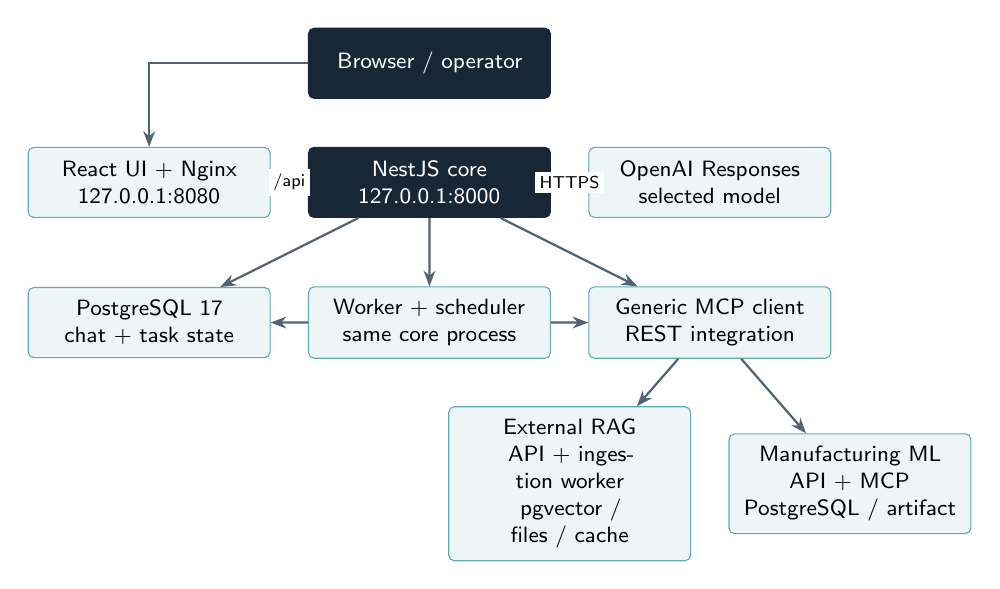
\begin{tikzpicture}[scale=.89,transform shape]
\node[darkbox] (browser) at (0,6.3) {Browser / operator};
\node[box] (ui) at (-4,4.6) {React UI + Nginx\\127.0.0.1:8080};
\node[darkbox] (core) at (0,4.6) {NestJS core\\127.0.0.1:8000};
\node[box] (llm) at (4,4.6) {OpenAI Responses\\selected model};
\node[box] (db) at (-4,2.6) {PostgreSQL 17\\chat + task state};
\node[box] (task) at (0,2.6) {Worker + scheduler\\same core process};
\node[box] (mcp) at (4,2.6) {Generic MCP client\\REST integration};
\node[box] (rag) at (2,.3) {External RAG\\API + ingestion worker\\pgvector / files / cache};
\node[box] (ml) at (6,.3) {Manufacturing ML\\API + MCP\\PostgreSQL / artifact};
\draw[arr] (browser) -| (ui);\draw[arr] (ui) -- node[lab]{/api} (core);
\draw[arr] (core) -- node[lab]{HTTPS} (llm);
\draw[arr] (core) -- (task);\draw[arr] (core) -- (db);
\draw[arr] (task) -- (db);\draw[arr] (core) -- (mcp);
\draw[arr] (task) -- (mcp);\draw[arr] (mcp) -- (rag);\draw[arr] (mcp) -- (ml);
\end{tikzpicture}
\captionof{figure}{Complete runtime boundary. The RAG and manufacturing stacks have their own persistent stores; OpenAI inference is remote.}\end{center}
\begin{tabularx}{\linewidth}{@{}lXl@{}}\toprule
Component & Implementation / responsibility & Host port\\\midrule
UI & React 19, Vite 8, Tailwind 4, shadcn; Nginx & 8080\\
Core & NestJS 12, Node 24, \texttt{pg}; chat/MCP/tasks & 8000\\
Chat database & PostgreSQL 17; messages, files, task ledgers & private\\
RAG & Python 3.12+, FastAPI, pgvector; API/worker & 8090\\
Manufacturing & FastAPI, scikit-learn, joblib; ML/MCP & 8100\\\bottomrule
\end{tabularx}
\section{Why one core and independent services?}
The existing core process runs both the task worker and scheduler. PostgreSQL locking supplies concurrency control; no separate broker or queue microservice is introduced. External services retain their own databases, models and files. The shared \texttt{meta-harness-mcp} bridge enables container-to-container connections, while published application ports bind to loopback.

The main Compose stack builds three images. Core includes compiled TypeScript and immutable migrations; the secret file is mounted only at runtime. UI assets contain no connection credentials. \texttt{App.tsx} preserves the chat/draft while management pages replace the main content area. LLM text is not streamed token by token; task status uses SSE and polling.
\source{\path{core/src/app.module.ts}; \path{ui/src/App.tsx}; \path{docker-compose.yml}; \path{docker-compose.mcp.yml}; \path{core/Dockerfile}; \path{ui/Dockerfile}.}

\chapter{Agent Harness and Execution Loop}
\partlabel{PART II --- AGENT ENGINEERING}
\section{Initialization and context construction}
Nest imports the chat, LLM, MCP, RAG and task modules. Startup loads root environment configuration, initializes PostgreSQL and applies migrations before workers claim tasks. The saved provider/key/model/thinking settings are reused for both chat and durable execution. There is one reasoning-model integration, not a separate task agent.

Ordinary chat enters \texttt{LlmService.respond()}. It builds provider function definitions from currently enabled, connected and allowlisted MCP tools. Responses may contain function calls; the loop resolves the generated function name, validates arguments, performs permitted execution and appends a \texttt{function\_call\_output}. A final text response ends the ordinary loop.

A durable task instead enters \texttt{TaskWorker.run()}. It reconstructs task state, prepares an incremental snapshot and calls \texttt{taskDecision()}. The system instructions in \texttt{task-prompt.ts} ask for one structured decision: execute, wait, complete, blocked or respond. Each worker slice performs at most one selected action, then commits a checkpoint before another slice is claimed.
\begin{center}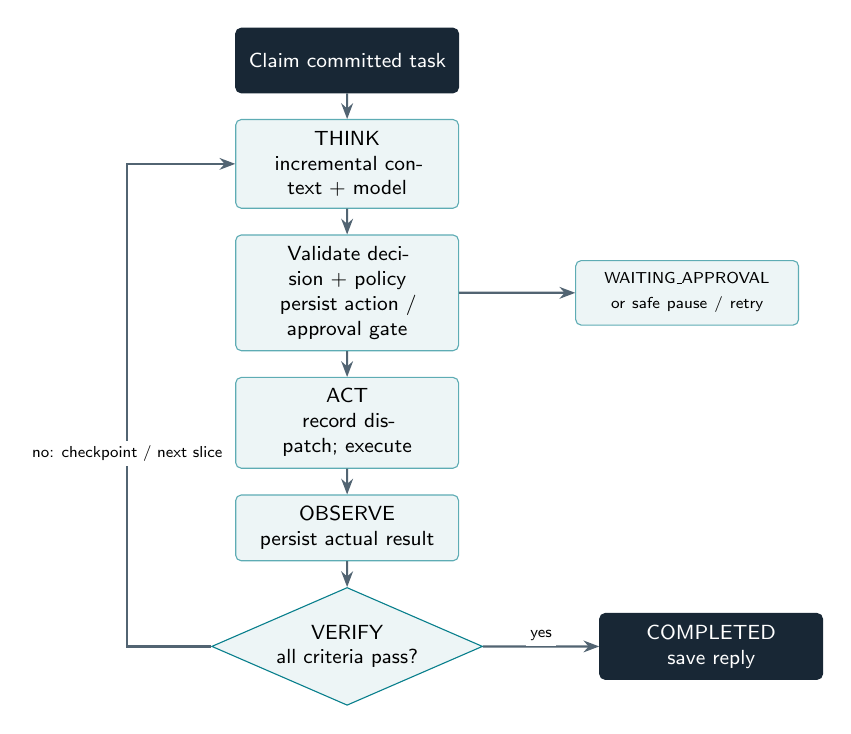
\begin{tikzpicture}[scale=.82,transform shape,node distance=4mm]
\node[darkbox] (claim) {Claim committed task};
\node[box,below=of claim] (think) {THINK\\incremental context + model};
\node[box,below=of think] (policy) {Validate decision + policy\\persist action / approval gate};
\node[box,below=of policy] (act) {ACT\\record dispatch; execute};
\node[box,below=of act] (obs) {OBSERVE\\persist actual result};
\node[decision,below=of obs] (verify) {VERIFY\\all criteria pass?};
\node[darkbox,right=18mm of verify] (done) {COMPLETED\\save reply};
\draw[arr] (claim)--(think);\draw[arr] (think)--(policy);\draw[arr] (policy)--(act);\draw[arr] (act)--(obs);\draw[arr] (obs)--(verify);
\draw[arr] (verify)--node[lab,above]{yes} (done);
\draw[arr] (verify.west)--++(-1.3,0) |- node[lab,pos=.2]{no: checkpoint / next slice} (think.west);
\node[box,right=18mm of policy] (approval) {\scriptsize WAITING\_APPROVAL\\or safe pause / retry};
\draw[arr] (policy)--(approval);
\end{tikzpicture}
\captionof{figure}{Durable THINK--ACT--OBSERVE--VERIFY--CONTINUE loop. Policy and evidence checks are backend decisions.}\end{center}
\section{Structured decisions are executable proposals}
The JSON schema includes a goal, ordered plan, measurable criteria, zero-based plan step, action and human summary. A proposed MCP action contains the real registered server UUID, tool name and argument object. Tool metadata is data, not authority. Instructions encourage conservative assumptions for vague objectives, but the backend does not translate vagueness into write permission.

\texttt{parseTaskDecision()} scans quoted/escaped JSON safely, validates with Ajv and parses nested argument/filter JSON. Identical execute/wait duplicates can be collapsed; conflicting or malformed decisions are rejected before dispatch. Response parsing is bounded to 262,144 characters and 512 objects. The raw redacted model output is retained separately for diagnosis.
\source{\path{core/src/llm/llm.service.ts}: \texttt{respond()}, \texttt{taskDecision()}; \path{core/src/tasks/task-prompt.ts}; \path{core/src/tasks/task-decision-parser.ts}: \texttt{parseTaskDecision()}; \path{core/src/tasks/task-worker.ts}: \texttt{run()}.}
\nextpage{Continuation, stopping and cancellation}
\section*{Pseudocode derived from the worker}
\begin{lstlisting}
claim due task + advisory lock + lease owner
while one bounded worker slice is active:
    restore committed goal, criteria, pending action, context
    if hard cost/continuation cap exhausted: pause
    if prompt budget exhausted: summarize, checkpoint, requeue
    if no pending action:
        build incremental context; obtain one valid decision
        commit decision, private window and delivery cursors
    if respond/complete: verify stored evidence before completion
    if blocked: pause with explanation
    if wait: checkpoint and schedule next slice
    if execute:
        enforce current tool/workspace policy
        reuse completed write; request approval if required
        commit DISPATCHING before sending
        persist observation; verify; checkpoint and requeue
on interruption: pause uncertain writes; retry safe reads
release lease/advisory lock
\end{lstlisting}
\section*{Budgets have different purposes}
Ordinary chat has eight provider rounds, twelve tool calls and a two-minute deadline per prompt. A persisted continuation lets the existing UI automatically request the next prompt, up to twenty continuations per UI run. Three consecutive deadline prompts without progress pause for retry. A confirmation gate suspends continuation until the exact invocation is approved.

Durable tasks continue in core without browser requests. Defaults are eight decision attempts, 200,000 provider tokens and 120,000 active milliseconds per prompt, with twenty automatic checkpoints per task. \texttt{TASK\_MAX\_TURNS}, \texttt{TASK\_MAX\_TOKENS}, \texttt{TASK\_MAX\_ACTIVE\_MS} and \texttt{TASK\_MAX\_CONTINUATIONS} are operator overrides. A slice still has a two-minute abort deadline. Lifetime accounting and optional cost caps survive every checkpoint.

These bounds prevent indefinite execution; they do not prove progress. A completed operation can be followed by an unsuccessful verification or a poor next decision. Repeated provider/tool failures exhaust the bounded retry policy. Authentication and unsafe configuration failures stop instead of silently generating success.
\section*{What cancellation means}
Pause/cancel changes persisted state and revokes the running owner's ability to commit another fenced step. Heartbeats detect lease loss and abort local execution. A request already sent to an external service cannot be undone by cancellation. If an interrupted write may have executed, its outcome must be reconciled before reuse or retry. Cancelled and completed tasks are terminal in the control API.
\note{Observations and final output}{Tool results are committed independently of the final reply. Every task-owned chat message has a live status/output card. The UI stays in chat and offers an optional link to task details. A useful response can be delivered without tools; that verifies delivery only, not external work.}
\source{\path{core/src/tasks/task-worker.ts}: \texttt{claim()}, \texttt{fenced()}, \texttt{run()}, \texttt{advance()}, \texttt{continuePrompt()}; \path{core/src/tasks/tasks.service.ts}: \texttt{control()}; \path{ui/src/components/chat/task-feedback.tsx}.}

\chapter{Memory and State Persistence}
\section{Four forms of continuity}
A chat transcript and an execution checkpoint solve different problems. The transcript records what participants said. A checkpoint records what the runtime has actually committed, including pending or completed actions. RAG provides separately managed knowledge; it is not a hidden copy of conversation memory.
\begin{center}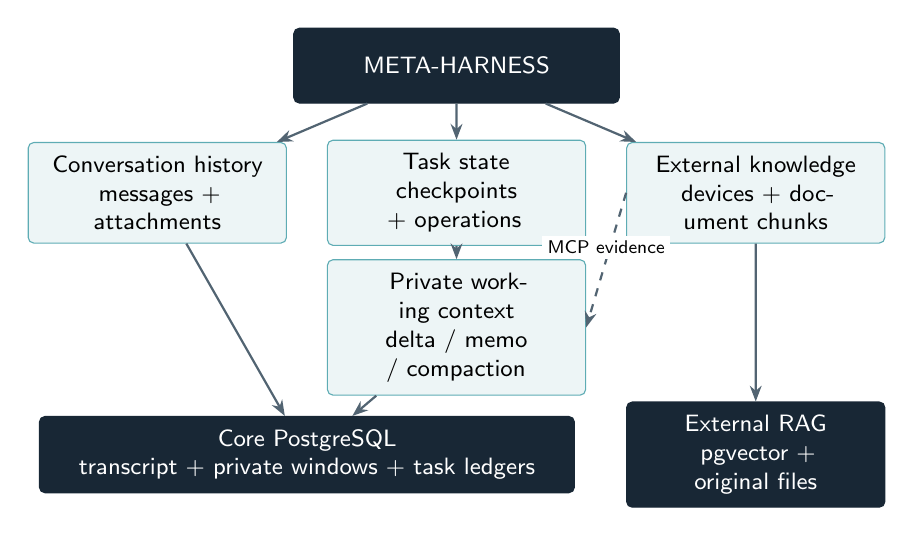
\begin{tikzpicture}[scale=.95,transform shape]
\node[darkbox,text width=4cm] (root) at (0,5.4) {META-HARNESS};
\node[box] (conv) at (-4,3.7) {Conversation history\\messages + attachments};
\node[box] (task) at (0,3.7) {Task state\\checkpoints + operations};
\node[box] (rag) at (4,3.7) {External knowledge\\devices + document chunks};
\node[box] (working) at (0,1.9) {Private working context\\delta / memo / compaction};
\node[darkbox,text width=6.8cm] (pg) at (-2,.2) {Core PostgreSQL\\transcript + private windows + task ledgers};
\node[darkbox] (rpg) at (4,.2) {External RAG\\pgvector + original files};
\draw[arr] (root)--(conv);\draw[arr] (root)--(task);\draw[arr] (root)--(rag);
\draw[arr] (conv)--(pg);\draw[arr] (task)--(working);\draw[arr] (working)--(pg);\draw[arr] (rag)--(rpg);
\draw[arr,dashed] (rag.west) -- node[lab,above]{MCP evidence} (working.east);
\end{tikzpicture}
\captionof{figure}{Memory ownership. Chat and task state share core PostgreSQL. External knowledge remains in the independent RAG database and file volumes.}\end{center}
\begin{description}
\item[Conversation memory] Ordered user/assistant messages, automatically derived chat titles, attachment bytes and compact tool traces. Saved messages remain visible even when model context is summarized.
\item[Working memory] The private input window supplied to the selected model: relevant messages, decisions, observations and opaque provider compaction/reasoning items. This is separate from UI text.
\item[Persistent task state] Goal, immutable plan/criteria, current and completed steps, pending action, operation ledger, approvals, retries, verification evidence, context cursors, budget baselines and lease information.
\item[Long-term domain knowledge] Device/issue data and searchable document passages in RAG. The agent retrieves relevant evidence through permitted MCP calls; it does not learn every uploaded manual permanently.
\end{description}
\section{Conversation reconstruction}
\texttt{ChatsService} inserts messages and attachments transactionally, serializes response generation per chat and links a reply to its originating user message. The unique reply linkage prevents multiple final replies to the same turn. Ordinary model context has a model identifier, complete private input items and a message-position watermark. Only new input is added when that saved window is compatible; model changes rebuild from visible input.

Attachments are stored as PostgreSQL \texttt{bytea} for downloading. Ordinary attachment content is not extracted into LLM context. Uploading a PDF with the chat plus button is therefore different from uploading it into RAG Documents.
\source{\path{core/src/chats/chats.service.ts}; \path{core/src/llm/context-window.ts}: \texttt{ChatContextWindow}; \path{database/schema.sql}; \path{ui/src/components/chat/attachment-card.tsx}.}
\nextpage{What PostgreSQL actually saves}
\section*{The core persistence model}
Core uses parameterized \texttt{pg} SQL, not an ORM. The schema snapshot and ordered migrations are applied inside a transaction with a database advisory lock. \texttt{schema\_migrations} stores a checksum for each upgrade; changing an applied migration is a startup error rather than an implicit schema rewrite.
\begin{tabularx}{\linewidth}{@{}lX@{}}\toprule
Entity & Persisted purpose\\\midrule
\texttt{chats} & Title, activity timestamps and private conversation context\\
\texttt{messages} & Role/text, order, reply linkage, tool traces and continuation state\\
\texttt{attachments} & Filename, MIME metadata, size and original bytes\\
\texttt{mcp\_servers} & Endpoints, discovered tools, permissions, status and credential-variable reference\\
\texttt{agent\_tasks} & Request/goal/plan/criteria, progress, next action, private context and budgets\\
\texttt{task\_steps} & Ordered decisions and execution step status\\
\texttt{task\_operations} & Stable operation identity, action, policy digest, dispatch/result/error and attempts\\
\texttt{task\_approvals} & Exact operation/action, policy identity and operator decision\\
\texttt{task\_verifications} & Criterion ID, pass/fail and actual observed evidence\\
\texttt{task\_events} & Sequenced progress/model/error/checkpoint events\\
\texttt{task\_schedules} & Cron/one-time schedule, timezone and task template\\\bottomrule
\end{tabularx}
Historical \texttt{task\_triggers} and \texttt{task\_trigger\_events} tables remain in the immutable schema but are inactive. Secrets are absent from these tables: profiles point to names in root \texttt{.env}.
\section*{State is saved before it becomes external work}
The worker first commits a model decision as \texttt{next\_action}. It then persists an operation identity and approval requirement. Immediately before sending a permitted external request, it commits \texttt{DISPATCHING}. Actual results, verification and progress are separate transactions. This ordering allows recovery to distinguish an unsent proposal from an action whose outcome is uncertain.

\texttt{fenced()} locks the task row and verifies RUNNING status plus the current lease-owner UUID. A stale worker cannot overwrite a pause/cancel or another owner's checkpoint. A session advisory lock supplies additional exclusion even if lease time expires while a process is still alive.
\section*{Schema evolution}
Migration 001 adds durable tasks, 002 adds estimated-cost accounting and 003 adds context-delivery state, prompt-token/turn/active-time baselines and a continuation counter. Task-operation evidence stays in PostgreSQL across all three. Foreign keys and cascade rules prevent orphaned task history when its conversation is deleted.
\source{\path{core/src/database/database.service.ts}: \texttt{onModuleInit()}, \texttt{transaction()}; \path{database/migrations/001_durable_tasks.sql}; \path{database/migrations/002_task_cost_budget.sql}; \path{database/migrations/003_task_context_checkpoints.sql}; \path{core/src/tasks/task-worker.ts}: \texttt{fenced()}.}
\nextpage{Incremental context and long-task continuity}
\section*{Why full snapshots were replaced}
The old task planner appended recent chat plus every full tool result on each turn. The private window grew with repeated evidence, while cumulative token limits could stop a task before its final source check. The current design separates authoritative storage from what the next model prompt needs.

\texttt{taskContextDelta()} fingerprints each operation's status, result, error and attempt count. A new prompt receives recent conversation and current tool schemas once. Later turns receive only changed operation observations and changed schemas, plus a bounded ledger and deterministic criterion statuses. Fingerprints and the resulting private window are committed together: a crash cannot mark evidence as delivered without saving the context that received it.
\section*{Bounded results with exact evidence access}
Each changed result is sent in full up to 12,000 characters; larger results use a marked preview. An update targets at most 64,000 characters of changed evidence, with pending changes delivered later. The ledger includes the latest forty operations; completed-step labels include the latest ten. Full original results remain in storage.

If exact detail is needed, the model chooses an internal \texttt{evidence} action. \texttt{readTaskEvidence()} resolves only operation IDs belonging to that task and applies a JSON pointer plus bounded offset/limit. It returns at most fifty array items or 12,000 text characters, also bounding large array pages. A nested oversized item can be inspected through a more specific pointer. This is neither an external replay nor a new proof of external execution.
\section*{Two distinct summarization boundaries}
\begin{enumerate}
\item Before inference, core counts the current model input. At 90\% of configured context capacity, the selected model's Responses compaction endpoint produces a canonical replacement window. If compaction remains too large or unavailable, original evidence is retained and an error is surfaced.
\item At a task prompt's turn/token/active-time budget, \texttt{summarizeTaskContext()} asks the same selected model for a factual working memo, with a 2,048-token output bound. \texttt{continuePrompt()} commits that memo, refreshes budget baselines and automatically requeues the task.
\end{enumerate}
The memo preserves identifiers, goals, sources, constraints, uncertain/declined writes and next steps. Immutable criteria and operation identities remain in database fields rather than depending solely on summary prose. Legacy windows receive one checkpoint when resumed. A failed summary does not replace the old window.
\note{What remains limited}{Summaries can omit facts or lose nuance. Exact stored-evidence reads mitigate loss but do not guarantee perfect model recall. Tokens/cost are cumulative; cost and continuation caps pause execution. Interrupted provider requests may be billed even when usage is unavailable. No semantic search over chat memory or learned personal-memory store is implemented.}
\source{\path{core/src/tasks/task-context.ts}: \texttt{taskContextDelta()}, \texttt{readTaskEvidence()}; \path{core/src/llm/llm.service.ts}: \texttt{summarizeTaskContext()}; \path{core/src/llm/context-window.ts}: \texttt{countContext()}, \texttt{compactContext()}.}

\chapter{Long-Running Tasks and Recovery}
\section{The worker is a durable database consumer}
The worker polls once per second. Default concurrency is two slices, configurable up to four. \texttt{claim()} selects due PENDING/RETRYING tasks or RUNNING tasks with expired leases using \texttt{FOR UPDATE SKIP LOCKED}. A session advisory lock prevents another live process from executing the same task; the committed owner UUID fences subsequent state changes. A heartbeat runs every five seconds and extends a thirty-second lease.

After a container restart, unfinished tasks are not reconstructed from a generated answer. They are reconstructed from persisted fields, the private window and operation states. An interrupted read is marked failed and may safely retry. An interrupted dispatched write becomes UNKNOWN and pauses for reconciliation. The worker never assumes the external service rolled back with the core process.
\begin{center}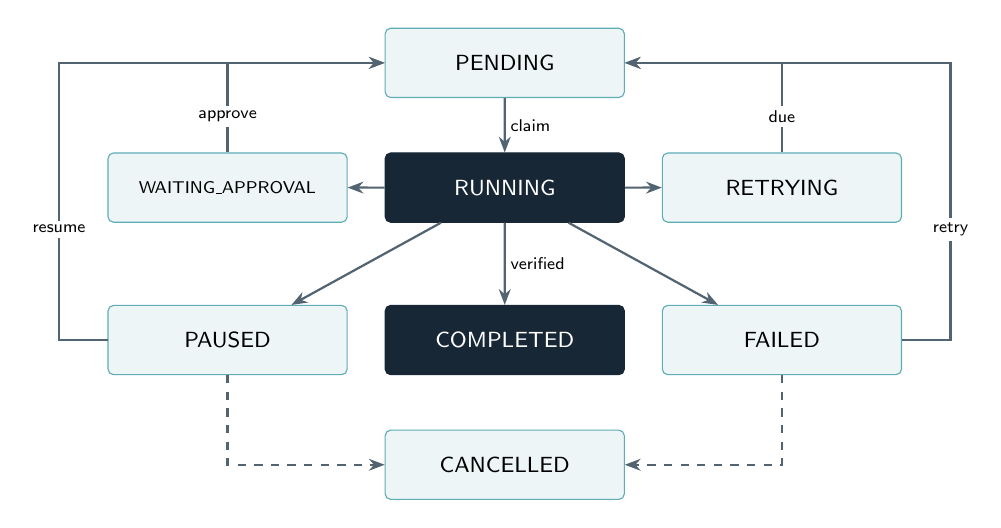
\begin{tikzpicture}[scale=.88,transform shape]
\node[box] (pending) at (0,4.6) {PENDING};
\node[darkbox] (running) at (0,2.8) {RUNNING};
\node[box] (approval) at (-4,2.8) {\scriptsize WAITING\_APPROVAL};
\node[box] (retry) at (4,2.8) {RETRYING};
\node[box] (pause) at (-4,.6) {PAUSED};
\node[darkbox] (done) at (0,.6) {COMPLETED};
\node[box] (fail) at (4,.6) {FAILED};
\node[box] (cancel) at (0,-1.2) {CANCELLED};
\draw[arr] (pending)--node[lab,right]{claim} (running);
\draw[arr] (running)--(approval);\draw[arr] (approval.north) |- node[lab,pos=.2]{approve} (pending.west);
\draw[arr] (running)--(retry);\draw[arr] (retry.north) |- node[lab,pos=.2]{due} (pending.east);
\draw[arr] (running)--node[lab,right]{verified} (done);
\draw[arr] (running)--(pause);\draw[arr] (running)--(fail);
\draw[arr] (pause.west)--++(-.7,0) |- node[lab,pos=.2]{resume} (pending.west);
\draw[arr] (fail.east)--++(.7,0) |- node[lab,pos=.2]{retry} (pending.east);
\draw[arr,dashed] (pause.south) |- (cancel.west);\draw[arr,dashed] (fail.south) |- (cancel.east);
\end{tikzpicture}
\captionof{figure}{Task lifecycle. UNKNOWN is an operation state; it causes a PAUSED task. Completion requires evidence verification.}\end{center}
\section{Retries are classified, bounded and recorded}
Transient provider/network/service errors use exponential backoff with jitter. \texttt{retryDelay()} starts from a one-second base, doubles by attempt, caps its base at five minutes and respects a returned Retry-After interval. The jitter multiplier is 0.75--1.25. The configured retry count defaults to five retries after the initial failing attempt.

A read-only MCP tool-level rejection saves the original error result, clears the failed pending action and asks the model for a corrected decision. The model can resolve a real device UUID instead of repeating a rejected name filter. Authentication, invalid policy/configuration and other permanent failures stop. Connection rediscovery is limited to enabled, permitted profiles that were not manually disconnected.
\source{\path{core/src/tasks/task-worker.ts}: \texttt{claim()}, \texttt{tick()}, \texttt{run()}; \path{core/src/tasks/task-contract.ts}: \texttt{retryDelay()}; \path{core/src/tasks/tasks.service.ts}: \texttt{control()}, \texttt{reconcile()}.}
\nextpage{Idempotency, schedules and operator recovery}
\section*{Stable identities protect completed writes}
A task operation has a stable UUID and unique task/operation key. Read actions use step plus canonical action identity. Writes are bound to a stable plan step or canonical arguments; an already successful canonical write is reused rather than executed again. The backend rechecks current configuration and permissions immediately before dispatch.

For durable MCP calls, core sends the UUID in \texttt{Idempotency-Key} and MCP \texttt{\_meta.operationId}. Remote services may ignore these fields. The implementation therefore provides ledger-based replay prevention and conservative uncertainty handling; it does not claim exactly-once external execution.
\begin{tabularx}{\linewidth}{@{}lX@{}}\toprule
Operation state & Recovery interpretation\\\midrule
PREPARED & A persisted proposal; no dispatch recorded\\
DISPATCHING & Send may have occurred; a restarted write becomes UNKNOWN\\
SUCCEEDED & Actual result recorded; successful writes are reused\\
FAILED & A recorded failure; retry policy depends on operation safety\\
UNKNOWN & External write outcome unresolved; operator checks the service\\
REJECTED & Operator declined the action; no automatic repetition\\\bottomrule
\end{tabularx}
\section*{Reconciliation is not invented evidence}
Task details can record ``Succeeded externally'' or ``Definitely not executed'' after the operator inspects the remote system. A reason is persisted. This resolves replay safety, but reconciliation-marked results are excluded from completion evidence; fresh reads must establish the outcome. Cancellation does not reverse a remote training/upload already sent.
\section*{Persistent schedules}
\texttt{TaskSchedulesService} supports future one-time dates and cron expressions with IANA timezones. It transactionally creates the occurrence task and advances the schedule. A unique key formed from schedule ID and scheduled time prevents duplicate creation. Missed recurring occurrences coalesce into one catch-up task; the next recurrence is calculated from current time. Invalid templates are disabled with an explanation, preventing a bad schedule from repeatedly starving other work.

Scheduled tasks keep their configured scope and permission grants. The UI schedule form does not provide broad automatic write grants; state-changing actions therefore ask for approval. A user initiating a request alone is not unlimited authorization.
\note{Event-driven status}{\status{REMOVED FOR NOW}: trigger navigation, configuration endpoints, webhook intake, task-completion publication and event dispatch. Historical tables remain inert. Earlier event-authentication tests document an older capability, not the current product. Do not configure a trigger through an undocumented route.}
\note{Recorded restart evidence}{The isolated SIGKILL fixture interrupted a read after a committed MCP write. Its recorded outcome was COMPLETED, with one write and two read attempts. The fixture used the real worker/PostgreSQL/MCP SDK and a deterministic planner. It was not rerun for this manual~\cite{recoveryrecord}.}
\source{\path{core/src/tasks/task-schedules.service.ts}: \texttt{save()}, \texttt{tick()}, \texttt{nextCron()}; \path{core/src/tasks/tasks.service.ts}: \texttt{reconcile()}; \path{core/tests/task-restart-review.py}; \path{docs/verification/task-restart.json}.}

\chapter{Security and Permission Management}
\section{The model proposes; core authorizes}
System prompts describe safe behavior, but permission enforcement lives in TypeScript. A discovered tool must belong to an enabled, connected profile, be explicitly allowlisted and be enabled for agent use. Its name/schema are revalidated before execution. A server description is untrusted content, not a grant of authority.
\begin{center}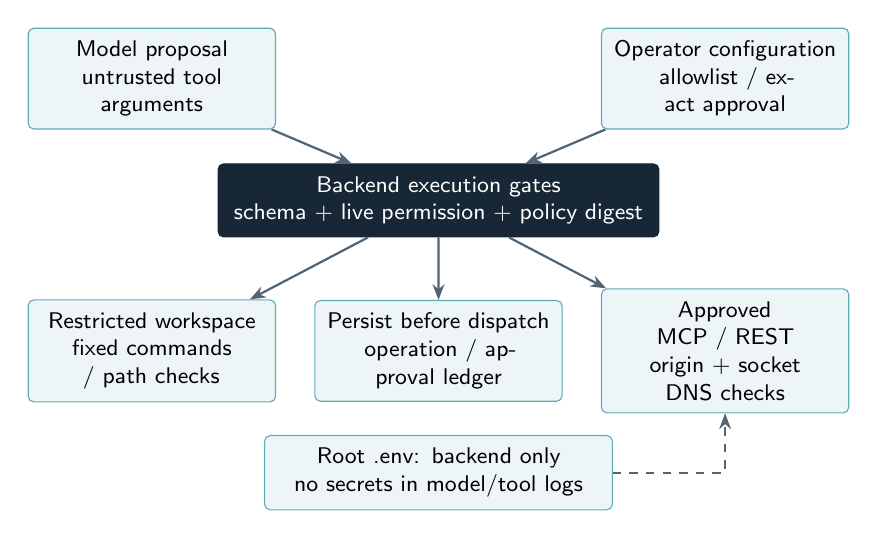
\begin{tikzpicture}[scale=.91,transform shape]
\node[box] (model) at (-4,4.4) {Model proposal\\untrusted tool arguments};
\node[box] (operator) at (4,4.4) {Operator configuration\\allowlist / exact approval};
\node[darkbox,text width=5.8cm] (gate) at (0,2.7) {Backend execution gates\\schema + live permission + policy digest};
\node[box] (workspace) at (-4,.6) {Restricted workspace\\fixed commands / path checks};
\node[box] (remote) at (4,.6) {Approved MCP / REST\\origin + socket DNS checks};
\node[box] (ledger) at (0,.6) {Persist before dispatch\\operation / approval ledger};
\draw[arr] (model)--(gate);\draw[arr] (operator)--(gate);\draw[arr] (gate)--(workspace);\draw[arr] (gate)--(remote);\draw[arr] (gate)--(ledger);
\node[box,text width=4.5cm] (secrets) at (0,-1.1) {Root .env: backend only\\no secrets in model/tool logs};
\draw[arr,dashed] (secrets.east) -| (remote.south);
\end{tikzpicture}
\captionof{figure}{Trust and execution gates. Secrets remain in backend configuration; external content does not bypass policy.}\end{center}
\section{Three backend permission levels}
\begin{description}
\item[Safe] Read/list/exists within the configured workspace and narrowly parsed read-only commands. Permitted read-only MCP tools may run without interrupting the operator.
\item[Controlled] Workspace writes and operator-classified MCP writes. A write needs exact approval, or an explicit per-task grant for an eligible MCP tool. A prompt is not a broad grant.
\item[Dangerous] Single-file deletion, explicitly dangerous MCP tools and unclassified state-changing MCP tools. These always require exact approval; task-wide grants cannot authorize them.
\end{description}
\texttt{TASK\_CONTROLLED\_MCP\_TOOLS} and \texttt{TASK\_DANGEROUS\_MCP\_TOOLS} contain reviewed server-UUID/tool bindings. A grant's digest includes endpoint, credential reference, allowlist and tool metadata, so configuration changes invalidate stale authority. Ordinary chat consumes a single-use confirmation before sending a write and rejects automatic replay of an interrupted confirmed call.
\section{Scope and residual trust}
The UI/core ports bind to loopback. Origin checks reject foreign browser mutation origins, but requests without an Origin header are accepted. This is a local operator application, not a multi-user production authorization service. MCP \texttt{readOnlyHint} is server-supplied; the operator must trust and review the service. No LLM prompt can guarantee that a malicious remote tool honors its hint.
\source{\path{core/src/tasks/execution-policy.ts}: \texttt{grant()}, \texttt{prepare()}; \path{core/src/mcp/mcp.service.ts}: \texttt{prepareCall()}, \texttt{execute()}; \path{core/src/config/local-origin.ts}: \texttt{requireLocalOrigin()}.}
\nextpage{Filesystem, network and secret protection}
\section*{Structured commands, not arbitrary shell execution}
Local tools are disabled until \texttt{TASK\_WORKSPACE\_ROOT} is set. The Docker workspace overlay mounts only an approved directory at \texttt{/workspace}; it does not expose the host Docker socket or the whole repository. Paths cannot escape through traversal or symlinks. Protected names include environment, credential and private-key files.

Commands use fixed binaries and parsed argument grammars, never \texttt{shell:true}. Supported examples are \texttt{pwd}, bounded \texttt{ls/find}, \texttt{cat} of one approved file, literal \texttt{grep -F}, \texttt{git status --short} and \texttt{git diff --stat}. Shell chaining, redirection, substitution and arbitrary SQL/Python are rejected. File reads/writes are bounded to 256 KiB; writes use temporary no-follow files and atomic rename. Execution uses a minimal environment without credentials, a ten-second timeout and bounded output. Git disables hooks/fsmonitor/external diff/text conversion.

The implementation provides application-level path and process restrictions, not a complete hostile-code sandbox. Complex compilation, dependency installation or Docker operations would require a separate operator-controlled MCP runner; none is built into core.
\section*{Outbound service connections}
\texttt{approvedUrl()} permits absolute HTTP(S) URLs only, without inline credentials, query or fragment, and requires an exact operator-approved origin. \texttt{guardedFetch()} rejects redirects/cross-origin requests and validates DNS addresses at actual socket lookup to reduce rebinding risk. Link-local/metadata and other unsafe address ranges are blocked. Approved loopback/private addresses remain usable for local services. External RAG operations are additionally constrained to known routes, methods and query names.
\section*{Credential lifecycle}
Passwords, API keys and tokens live in the ignored root \texttt{.env}. The core image never contains this file. Compose injects the database password and mounts only root \texttt{.env} into core for authorized settings writes. UI and database do not mount the secret file; frontend assets never receive tokens.

The LLM key entry saves a replacement once, clears the input and returns only the first four characters followed by stars. MCP/RAG tokens use generated \texttt{MCP\_TOKEN\_<UUID>} variables; database profiles keep the variable name, not a token. Reads expose saved-credential flags. Redaction filters traces/model outputs before publication. The screenshot copies in this manual hide the saved-key display completely.
\note{Injection and disclosure limits}{Tool descriptions and passages are treated as untrusted observations. Permissions, bounded schemas and network gates limit what malicious content can cause; they do not prove that model reasoning is immune to injection. Sending retrieved evidence to OpenAI remains a data-flow decision the local operator must accept. There is no external answer validator or general data-loss-prevention engine.}
\source{\path{core/src/tasks/execution-policy.ts}: \texttt{workspacePath()}, \texttt{execute()}; \path{core/src/mcp/network-policy.ts}: \texttt{approvedUrl()}, \texttt{guardedFetch()}; \path{core/src/config/environment-store.service.ts}; \path{core/src/rag/rag.controller.ts}: \texttt{validateOperation()}.}

\chapter{LLM and Tool Integration}
\section{LLM connection and provider compatibility}
The LLM sidebar stores the provider (OpenAI), replacement API key, model and thinking selection. \texttt{LlmService.models()} retrieves the authenticated provider model catalog; model discovery is not an inference test. A listed model can still reject Responses input, reasoning effort or structured output. Core converts provider errors to useful messages without exposing raw provider bodies.

\texttt{respond()} uses the Responses API with discovered function definitions and the selected reasoning setting. \texttt{taskDecision()} uses the same settings with a strict JSON-schema output named \texttt{task\_decision}. ``Instant'' maps to reasoning effort \texttt{none}; medium/high use their corresponding effort. A configured model must support the requested combination. No external model is introduced for planning, summaries or task recovery.
\section{Context construction is a backend operation}
For ordinary chat, a compatible private window receives only new messages and actual function-call outputs. Durable execution receives an incremental task snapshot containing authoritative progress and fresh evidence. Both count input before inference and compact at 90\% of configured capacity. \texttt{LLM\_CONTEXT\_WINDOW\_TOKENS} can override the source's known-model capacity mapping; otherwise an unrecognized model falls back to 128,000 tokens. A local sixteen-MiB guard bounds serialized context.

The normal system instructions stress source provenance, uncertain device identity, untrusted service content and that RAG ranking is not diagnostic confidence. Task instructions additionally define one-action decisions, immutable criteria and write authorization. These constraints guide model behavior; live policy checks still decide what can execute.
\section{Progress is not token streaming}
Responses are returned after completion. The UI displays Responding, retries or task status while work runs. Task events use \texttt{/api/tasks/stream} SSE, with polling fallback in chat. This is progress/status delivery, not a live stream of generated answer tokens.

A provider timeout, 429/rate-limit or temporary service failure can be retried according to the relevant chat/task path. Missing credentials, unsupported model combinations or refused context operations are surfaced explicitly. An interrupted paid request may still be charged. A failed response cannot silently replay a confirmed write.
\note{Model API versus harness}{The provider supplies reasoning and structured output. Core supplies durable identity, checkpoint consistency, tool permission, idempotency policy and verification. Changing the selected model changes capabilities and summary quality; it does not remove those backend gates.}
\source{\path{core/src/llm/llm.service.ts}: \texttt{configuration()}, \texttt{models()}, \texttt{save()}, \texttt{respond()}, \texttt{taskDecision()}; \path{core/src/llm/context-window.ts}: \texttt{contextBudget()}, \texttt{openAiRequest()}; \path{ui/src/components/llm/llm-settings.tsx}.}
\nextpage{MCP discovery and execution}
\section*{One registry, independently configurable services}
\texttt{mcp\_servers} stores the operator's name/description, URL, enabled flags, discovered tools, allowlist, last error and authentication-variable reference. RAG adds REST metadata to the same profile rather than introducing a competing registry. Core reconnects enabled agent profiles at startup, except those explicitly disconnected.

\texttt{inspect()} opens an official TypeScript MCP SDK client over Streamable HTTP, initializes the connection and paginates \texttt{listTools}. Discovery is bounded to 500 tools, two MiB of catalog data and 64 KiB per input schema. The discovery deadline is fifteen seconds. Server name and metadata come from the actual server, not the description field.

\texttt{agentTools()} publishes at most sixty-four currently permitted definitions. Each generated function name hashes server UUID plus tool name, preventing same-named tools on different servers from overwriting one another. Descriptions combine the server purpose and actual tool description; parameters use the discovered input schema.
\begin{center}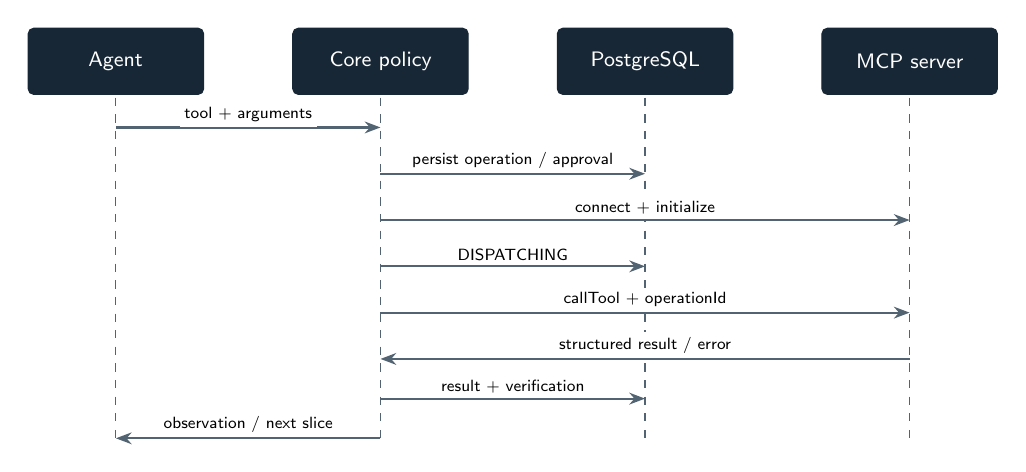
\begin{tikzpicture}[scale=.84,transform shape]
\foreach \name/\x/\label in {agent/0/Agent,core/4/Core policy,db/8/PostgreSQL,server/12/MCP server}{\node[darkbox,text width=2.3cm] (\name) at (\x,0) {\label};\draw[muted,dashed] (\x,-.55)--(\x,-5.7);}
\draw[arr] (0,-1)--node[lab,above]{tool + arguments} (4,-1);
\draw[arr] (4,-1.7)--node[lab,above]{persist operation / approval} (8,-1.7);
\draw[arr] (4,-2.4)--node[lab,above]{connect + initialize} (12,-2.4);
\draw[arr] (4,-3.1)--node[lab,above]{DISPATCHING} (8,-3.1);
\draw[arr] (4,-3.8)--node[lab,above]{callTool + operationId} (12,-3.8);
\draw[arr] (12,-4.5)--node[lab,above]{structured result / error} (4,-4.5);
\draw[arr] (4,-5.1)--node[lab,above]{result + verification} (8,-5.1);
\draw[arr] (4,-5.7)--node[lab,above]{observation / next slice} (0,-5.7);
\end{tikzpicture}
\captionof{figure}{A durable MCP call. The database dispatch checkpoint precedes the remote call; output remains traceable to server/tool/operation.}\end{center}
\section*{Execution and observation handling}
\texttt{prepareCall()} validates current enablement, allowlisting, schema and bounded object arguments using Ajv. Regex-pattern schemas are currently unsupported. \texttt{execute()} initializes a session, rechecks configuration identity, records dispatch and calls the tool. It bounds session time to twenty seconds, the call to fifteen seconds and normalized output to 256 KiB. The guarded transport bounds remote response bytes separately.

Results retain MCP content and structured content. Traces record server/tool, duration, success and source/result summaries without credentials. Tool-level \texttt{isError} is different from a network exception; read-only task rejections can be corrected using their actual stored observation. A failed connection gets a saved error state; manually disconnected or revoked tools cannot be silently re-enabled by the planner.
\source{\path{core/src/mcp/mcp.service.ts}: \texttt{onApplicationBootstrap()}, \texttt{inspect()}, \texttt{discover()}, \texttt{agentTools()}, \texttt{prepareCall()}, \texttt{execute()}; \path{core/src/llm/llm.service.ts} (chat continuation/trace types).}

\chapter{Validation and Completion Verification}
\section{A successful tool is only one piece of evidence}
A training API can successfully return a queued job while no artifact exists. Retrieval can successfully return no passages. A generated final answer can describe a plan without executing it. The harness therefore distinguishes transport success, operation success and completion of the user's objective.

The first durable decision proposes measurable completion criteria, faithful to the request. Core freezes the initial goal, plan and criteria when the first valid plan is committed. Subsequent decisions cannot silently weaken the criteria to make progress appear complete.
\section{Deterministic predicates over actual results}
\texttt{checkCriterion()} selects SUCCEEDED operations by kind, optional registered server/tool and exact argument filters. It excludes operator-reconciled placeholder outcomes. A JSON pointer selects an observed value from the stored result. Supported predicates are:
\begin{itemize}
\item \texttt{exists}: value is present and not null;
\item \texttt{equals}: canonical serialized equality to an expected value;
\item \texttt{nonempty}: nonblank string or nonempty array/object;
\item \texttt{gte}: numeric value meets an expected numeric threshold;
\item \texttt{contains}: substring or exact member of an array.
\end{itemize}
Filters accept explicit JSON pointers or plain exact property names. Each verification row records the criterion ID, result and observed operation/value evidence. Progress is the fraction of passed predicates, capped below 100 until completion; it is not a simulated processing percentage.
\section{What complete and respond mean}
\texttt{TasksService.complete()} runs verification and inserts the final assistant reply only when all criteria pass. The reply links to the original user message; the task becomes COMPLETED with a saved result. A model \texttt{complete} decision without evidence is insufficient and returns to continuation.

A \texttt{respond} decision can deliver a useful informational answer without tools. For a fresh response-only task, core creates an internal response operation and verifies nonempty delivery with \texttt{externalExecutionVerified} set to false. With existing external criteria, a partial answer stays visible but unmet criteria pause the task. A greeting or draft answer does not need fabricated tool execution.
\note{Validation limits}{Schema validity is not factual validity. A criterion such as ``result exists'' may be weaker than the intended semantic outcome; the model still chooses the initial tests. Core does not implement a universal diagnosis evaluator, PDF compilation runner or external answer validator. Stronger research workflows and validators remain planned.}
\source{\path{core/src/tasks/task-contract.ts}: \texttt{matches()}, \texttt{pointer()}, \texttt{checkCriterion()}; \path{core/src/tasks/tasks.service.ts}: \texttt{verify()}, \texttt{complete()}; \path{core/src/tasks/task-worker.ts}: \texttt{advance()}.}
\nextpage{Real example: CNC source verification}
\section*{The observed failure and correction}
A live CNC retrieval task initially passed the string ``Milling machine CNC'' into a \texttt{device\_id} filter. The external RAG MCP tool rejected the search as invalid. The rejected observation was retained, not interpreted as successful retrieval.

A corrected continuation resolved the device through \texttt{find\_device}, then successfully ran \texttt{search\_knowledge} and \texttt{get\_device\_issues}. Three checks passed, but the task still lacked its required source-context evidence. Repeated full snapshots exhausted the old aggregate token limit before that final step.
\section*{Checkpoint recovery produced actual completion}
After the context change, the authorized task was retried from saved state. The selected model summarized its legacy window once. Incremental snapshots then included only changed observations. The worker invoked the missing \texttt{get\_document\_context} and stored the final response. All four existing predicates passed~\cite{contextrecord}.
\begin{tabularx}{\linewidth}{@{}lX@{}}\toprule
Check & Recorded result after resumption\\\midrule
\texttt{device\_match} & Passed from stored device lookup evidence\\
\texttt{issues} & Passed from stored known-issue retrieval\\
\texttt{guidance} & Passed from successful knowledge search\\
\texttt{sources} & Passed after document-context retrieval\\\bottomrule
\end{tabularx}
The previously successful device lookup, search and issue calls each retained one attempt. The historical rejected search also remained at one attempt. Only the missing document-context call was added; this is observable continuity, not a claim based on model prose.
\section*{What the record proves, and what it does not}
The recorded task reached COMPLETED and 100\% verified progress. Its lifetime usage was 406,031 tokens, while the resumed prompt consumed 28,665 tokens after a 377,366-token baseline. These are operational accounting values, not a latency benchmark or a claim of general agent accuracy. The working-window capture shows conversation/tool schemas in the first new snapshot and neither in the next; the latter delivered only the new operation result.

The run exercised legacy summarization and incremental delivery. It did not reach another fresh prompt boundary, select internal evidence paging or test a new restart at the 90\% context threshold. Those limits are explicitly recorded. Earlier restart/concurrency fixtures validate a different execution scenario.
\note{Engineering interpretation}{Durability preserved evidence; context redesign avoided resending it; deterministic verification withheld completion until the missing source operation succeeded. The harness protects execution integrity, while relevance and adequacy still depend on retrieval quality and the initially chosen predicates.}
\source{\path{docs/verification/task-context-checkpoints.json}; \path{core/src/tasks/task-context.ts}; \path{core/src/tasks/task-worker.ts}: \texttt{continuePrompt()}; \path{core/src/tasks/tasks.service.ts}: \texttt{complete()}.}

\chapter{RAG and Knowledge Retrieval}
\partlabel{PART III --- RAG AND MANUFACTURING INTEGRATION}
\section{An independent retrieval service}
The RAG server is a standalone Python/FastAPI application, with SQLAlchemy, Alembic, PostgreSQL/pgvector, local HuggingFace embeddings and the Python MCP SDK. Its image runs either API/MCP or the ingestion worker. A separate pgvector-compatible database container and persistent document/model-cache volumes complete the stack. It has no chatbot, answer generation or OpenAI API requirement.
\begin{center}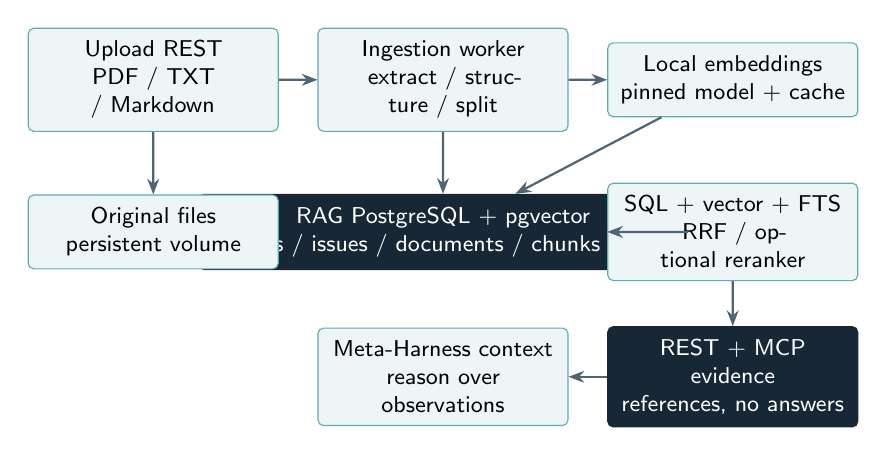
\begin{tikzpicture}[scale=.92,transform shape]
\node[box] (upload) at (-4,4.1) {Upload REST\\PDF / TXT / Markdown};
\node[box] (worker) at (0,4.1) {Ingestion worker\\extract / structure / split};
\node[box] (embed) at (4,4.1) {Local embeddings\\pinned model + cache};
\node[darkbox,text width=6.4cm] (db) at (0,2) {RAG PostgreSQL + pgvector\\devices / issues / documents / chunks / links};
\node[box] (files) at (-4,2) {Original files\\persistent volume};
\node[box] (search) at (4,2) {SQL + vector + FTS\\RRF / optional reranker};
\node[darkbox] (mcp) at (4,0) {REST + MCP evidence\\references, no answers};
\node[box] (agent) at (0,0) {Meta-Harness context\\reason over observations};
\draw[arr] (upload)--(worker);\draw[arr] (worker)--(embed);\draw[arr] (embed)--(db);\draw[arr] (upload)--(files);\draw[arr] (worker)--(db);\draw[arr] (db)--(search);\draw[arr] (search)--(mcp);\draw[arr] (mcp)--(agent);
\end{tikzpicture}
\captionof{figure}{RAG ingestion and retrieval. Only retrieved passages enter the agent's working context; original documents remain external.}\end{center}
\section{Six domain tables preserve relationships}
\texttt{devices} stores identity and metadata. \texttt{issues} stores symptoms, possible causes, text and automatically maintained embeddings. \texttt{documents} stores upload metadata, version and processing status, while original files remain in persistent storage. \texttt{device\_documents} associates a shared manual with multiple devices. \texttt{document\_chunks} preserves text, section path, page, order and vector. \texttt{issue\_evidence} explicitly links an issue and chunk with an evidence type.

Device identity uses UUIDs and constraints; names are not interchangeable with IDs. Possible causes are hypotheses, not confirmed faults. Evidence links are explicit operator relationships, not automatically inferred from semantic similarity.
\section{Uploads are durable work, not request-time indexing}
\texttt{DocumentService.upload()} validates references, extension/content type, size and UTF-8/PDF content, stores a UUID-based original filename and commits status \texttt{uploaded}. Content hashing supports duplicate handling. The HTTP response returns before embedding work. The worker selects due uploaded/interrupted/retryable documents, acquires a per-document lock and records attempts in document metadata; no seventh job-domain table is added.

Encrypted/corrupt or textless PDFs fail clearly. Scanned PDFs require external OCR before upload. Structure detection recognizes Markdown and simple text headings and preserves page provenance. These heuristics do not perfectly recover every technical layout.
\source{\path{rag-server/rag/models.py}; \path{rag-server/migrations/versions/0001_knowledge.py}; \path{rag-server/rag/documents.py}: \texttt{upload()}; \path{rag-server/rag/worker.py}: \texttt{run\_once()}, \texttt{process()}.}
\nextpage{Chunking, hybrid search and agent evidence}
\section*{Structure first, semantics second}
\texttt{extract()} reads PDF text or UTF-8 TXT/Markdown. \texttt{structures()} detects headings and marks warnings, steps and symptom/cause/solution blocks as protected. \texttt{Chunker.split()} applies LlamaIndex \texttt{SemanticSplitterNodeParser} inside sufficiently large unprotected sections, then enforces embedding-token bounds. Long procedures are packed by paragraph/step and warnings are repeated when a split is unavoidable.

The default embedding contract uses a pinned \texttt{all-MiniLM-L6-v2} revision and 384 dimensions. Local model initialization checks vector dimension; database/model-contract checks reject incompatible reconfiguration. Chunks retain embedding model metadata and document version. Cached local weights may require an initial network download; inference itself remains local. Offline mode requires a populated cache.

The worker stores replacement chunks and READY status in one transaction. Old chunks are deleted safely; foreign keys remove their explicit evidence links, which the operator must relink after reprocessing. Failures preserve status/error/attempt metadata and use bounded retries.
\section*{Complementary retrieval paths}
\texttt{RetrievalService.search()} resolves explicit or deterministic device identity, filters issues/documents through relational SQL and searches both issue vectors and full-text keywords. Matched issues contribute only their explicitly linked evidence. Direct document search works even when the device has no issues.

Document streams include cosine vector ranking, PostgreSQL English full-text ranking and linked issue evidence. Candidate UUIDs are deduplicated and fused by reciprocal rank:
\[
\operatorname{RRF}(d)=\sum_{r\in\mathcal R}\frac{1}{k+\operatorname{rank}_r(d)},\qquad k=60\ \text{by default}.
\]
An optional local cross-encoder reranks candidates when enabled. Output includes document/chunk IDs, title, section, page, device associations, matched issues, method and separate scores. Ranking values are not calibrated probabilities of a diagnosis.
\section*{How retrieved knowledge reaches the model}
The RAG MCP server exposes \texttt{find\_device}, \texttt{get\_device\_issues}, \texttt{search\_knowledge} and \texttt{get\_document\_context}. They reuse the same services as REST. Core exposes only discovered, explicitly selected read-only tools from this profile. Ordinary chat appends actual function-call observations; tasks store the full result and deliver an incremental preview or bounded exact evidence read.

The agent interprets these passages and reports sources. RAG supplies evidence, not a natural-language answer or an automatic proof of a fault. A vague device match, empty results or an unsupported manual can still leave the user's task incomplete.
\source{\path{rag-server/rag/chunking.py}: \texttt{extract()}, \texttt{structures()}, \texttt{Chunker.split()}; \path{rag-server/rag/embeddings.py}: \texttt{LocalEmbeddings}; \path{rag-server/rag/retrieval.py}: \texttt{search()}, \texttt{rrf()}; \path{rag-server/rag/mcp_server.py}: \texttt{build\_mcp()}.}

\chapter{Manufacturing ML Integration}
\section{A synthetic classifier, outside the harness}
The independent manufacturing stack has a private PostgreSQL database and one FastAPI ML/MCP image. Startup creates 1,000 reproducible synthetic products using seed 42, five machine codes and measured features: temperature, pressure, vibration, speed, humidity and material quality. The generator ties defect risk to these conditions with noise; it does not use unrelated random labels.

The persisted trusted artifact contains a scikit-learn StandardScaler/LogisticRegression pipeline, feature order, library version, model version, training metadata and evaluation fingerprint. \texttt{bundle()} rejects symlinks, foreign ownership or incompatible artifact metadata and caches by file identity/time. Joblib is loaded only from service-owned storage, not arbitrary uploads.
\section{Current label-removal boundary}
\status{IMPLEMENTED}: inference, dataset classification and metrics from the saved trained model. \status{UNAVAILABLE}: current retraining. \texttt{Product} no longer contains \texttt{quality\_label}; initialization removes that column. \texttt{train\_model()} now raises \texttt{TRAINING\_LABELS\_REMOVED}. Training submission/status tools remain discoverable, but discovery does not prove the operation can succeed. A clean volume cannot train a fresh model with the current code.

The separate frozen \texttt{evaluation\_products} snapshot retains 200 original feature/label rows. Predictions on production rows do not return ground-truth comparisons or overwrite measurements. A ground-truth label filter returns \texttt{LABELS\_REMOVED}; use predicted-label filtering for classification. Class convention remains 0 = Defective and 1 = Good.
\section{Actual results and tool abstraction}
Live read-only checks found the deployed model ready and 1,000 products. Its held-out accuracy was 0.67, precision 0.6869, recall 0.6602 and F1 0.6733, using Good as the positive class. The confusion matrix was $\left[\begin{smallmatrix}66&31\\35&68\end{smallmatrix}\right]$ with true-label rows and predicted-label columns in [Defective, Good] order. Metadata reported 800 training and 200 evaluation samples. These describe this synthetic artifact, not production manufacturing reliability~\cite{mlrecord}.
\begin{center}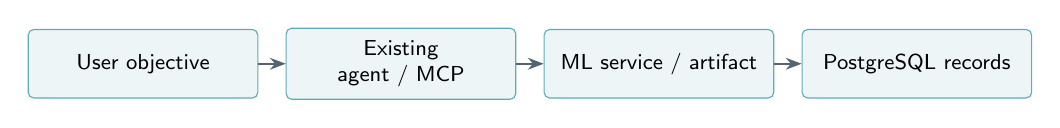
\begin{tikzpicture}[node distance=4mm,scale=.87,transform shape]
\node[box,text width=3cm] (a) {User objective};\node[box,text width=3cm,right=of a] (b) {Existing agent / MCP};\node[box,text width=3cm,right=of b] (c) {ML service / artifact};\node[box,text width=3cm,right=of c] (d) {PostgreSQL records};\draw[arr] (a)--(b);\draw[arr] (b)--(c);\draw[arr] (c)--(d);
\end{tikzpicture}\captionof{figure}{Read a bounded dataset, run actual inference and return structured predictions through the existing agent.}\end{center}
Six tools are exposed: dataset retrieval, training submission/status, product prediction, dataset classification and metrics. The agent registry contains no manufacturing-specific dispatch branch. Model probabilities are actual classifier outputs; they are not evidence that a named CNC machine has a particular fault.
\source{\path{manufacturing-demo/manufacturing/seed.py}: \texttt{synthetic\_records()}, \texttt{initialize()}; \path{manufacturing-demo/manufacturing/model.py}: \texttt{bundle()}, \texttt{predict()}, \texttt{train\_model()}; \path{manufacturing-demo/manufacturing/dataset.py}: \texttt{predictions()}; \path{manufacturing-demo/manufacturing/mcp_server.py}.}

\chapter{Installation and Configuration}
\partlabel{PART IV --- PRACTICAL USER GUIDE}
\section{Start the existing local stack}
\begin{enumerate}
\item Install Docker Engine with Compose v2. Native development additionally uses the repository's npm workspace dependencies; Docker builds use Node 24. RAG/ML builds need disk space for Python/model packages and initial internet access. Core inference needs OpenAI connectivity and an operator-provided key.
\item From the repository root, create \texttt{.env} only if absent. Set a strong \texttt{DB\_PASSWORD} locally. Preserve the password of an existing initialized database volume; changing the file alone does not update PostgreSQL's stored password.
\item Build/start the three-service application, then check its health.
\end{enumerate}
\begin{lstlisting}[language=bash]
test -e .env || cp .env.example .env
# Edit .env locally; keep all existing confidential entries.
chmod 600 .env
docker compose up --build -d --wait
curl http://127.0.0.1:8000/api/health
\end{lstlisting}
Open \url{http://localhost:8080}. The database is private; its \texttt{message-data} volume persists across ordinary restarts. Avoid deleting volumes. If external containers are already connected, retain the MCP overlay on subsequent core Compose commands (Chapter 12).
\section{Save the model connection}
\begin{minipage}[t]{.65\linewidth}
\begin{enumerate}
\item Expand \textbf{LLM}; company is currently OpenAI.
\item Enter a replacement API key and press \textbf{Save API key}. Input clears after submission. There is no reveal control.
\item Choose a model from the authenticated catalog; \textbf{Refresh} reloads it.
\item Choose \textbf{Instant}, \textbf{Medium} or \textbf{High} thinking, then \textbf{Save settings}.
\item Send a small ordinary message to confirm compatibility. Discovery alone does not prove text/structured-output support.
\end{enumerate}
For context-capacity overrides or cost limits, edit the root environment settings described in \path{docs/OPERATIONS.md} and \path{docs/TASK_EXECUTION.md}. Restart core after static worker/policy changes. Do not place tokens in frontend build variables.
\end{minipage}\hfill
\begin{minipage}[t]{.29\linewidth}\vspace{0pt}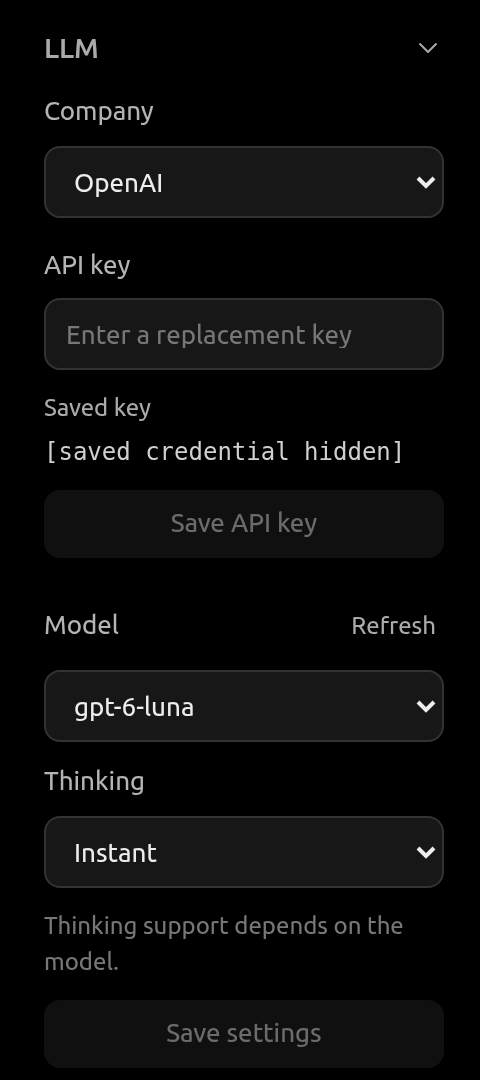
\includegraphics[width=\linewidth]{figures/ui-llm-panel.png}\captionof{figure}{Live LLM panel. Saved-key text hidden for publication.}\end{minipage}
\note{First-use checks}{New chat opens the existing composer. \textbf{+} stores/downloads ordinary attachments; it does not index them. Enter sends and Shift+Enter adds a line. Use \textbf{RAG → Documents} for searchable manual uploads.}
\source{\path{README.md}; \path{docker-compose.yml}; \path{.env.example}; \path{core/src/config/environment.ts}; \path{ui/src/components/llm/llm-settings.tsx}.}

\chapter{Connecting External Services}
\section{Generic MCP: configure, discover, allow}
\begin{enumerate}
\item Expand \textbf{MCP → Add MCP Server}. Enter a name, purpose description, absolute MCP URL and enabled state. For the containerized demonstration use \texttt{http://manufacturing-ml:8000/mcp}, not host localhost.
\item Choose None or Bearer Token. Enter a token once, or reference the existing root variable \texttt{MANUFACTURING\_API\_KEY}. No secret is stored in browser localStorage.
\item \textbf{Test Connection}, then \textbf{Save Connection}. Test/discover the saved profile. A changed draft must be saved before permissions can be granted.
\item Inspect actual discovered tools/descriptions/schemas. Select permitted tools, enable use in chat and \textbf{Save tool permissions}. Allow only the capabilities needed.
\item Use Connections to edit, enable/disable, disconnect or remove the profile. A disconnected profile is not silently reconnected by the worker.
\end{enumerate}
\screenshot{ui-mcp-add-current.png}{.88}{Genuine Add MCP Server view. Forms open in the main area; the chat layout and sidebar are preserved.}
\section*{Networking and standalone ML startup}
From the root, create \texttt{meta-harness-mcp} once if it does not exist; retain the overlay when recreating core. Set the demo's two secret variables locally before starting its stack.
\begin{lstlisting}[language=bash]
docker network create meta-harness-mcp  # once only
docker compose -f docker-compose.yml -f docker-compose.mcp.yml up -d --build
cd manufacturing-demo
docker compose --env-file ../.env -f docker-compose.yml \
  -f docker-compose.meta-harness.yml up -d --build --wait
\end{lstlisting}
Host clients use \texttt{localhost:8100/mcp}; core inside Docker uses the service URL. A clean manufacturing volume has no trainable production labels: preserve the trusted trained-artifact volume. If an origin is rejected, add its exact origin to root \texttt{MCP\_ALLOWED\_ORIGINS}; do not relax URL/DNS safety checks.
\source{\path{ui/src/components/mcp/mcp-workspace.tsx}: \texttt{ConnectionForm}; \path{core/src/mcp/mcp.controller.ts}; \path{manufacturing-demo/docker-compose.meta-harness.yml}; \path{docker-compose.mcp.yml}.}
\nextpage{RAG connection and knowledge management}
From \texttt{rag-server/}, with \texttt{RAG\_DB\_PASSWORD} and \texttt{RAG\_API\_KEY} set in root \texttt{.env}, start the independent stack:
\begin{lstlisting}[language=bash]
docker compose --env-file ../.env -f docker-compose.yml \
  -f docker-compose.meta-harness.yml up -d --build
\end{lstlisting}
\begin{enumerate}
\item In \textbf{RAG → Connection}, select an existing profile or New. For bridged Docker, use MCP \texttt{http://rag-api:8090/mcp} and separate REST \texttt{http://rag-api:8090}. Do not assume one URL can always be derived from the other.
\item Save authentication once; \textbf{Save Connection} and \textbf{Test Connection}. Inspect MCP and REST statuses independently. MCP-only connectivity enables retrieval; REST-only connectivity can still support management.
\item Select discovered read-only retrieval tools and enable their use in chat; \textbf{Save tool permissions}.
\end{enumerate}
\screenshot{ui-rag-current.png}{.83}{Live RAG connection: separate MCP and REST URLs and independently connected states. No token value is displayed.}
\begin{enumerate}[resume]
\item \textbf{Devices}: create an identity with name/model/manufacturer. \textbf{Documents}: upload PDF/TXT/Markdown, title/type/version and related devices. Wait for READY; status values are real, not fake percentages.
\item View document chunks and source pages. In \textbf{Known Issues}, add symptoms and a possible cause. Use evidence search to select a passage and an evidence type, rather than manually inventing chunk IDs.
\item In \textbf{Knowledge Search}, enter a query and optional device/category/top-k. Inspect matched issues and passages, expand IDs/method/scores, then return to chat. This page retrieves evidence without generating an LLM answer.
\end{enumerate}
\source{\path{ui/src/components/rag/connection.tsx}; \path{ui/src/components/rag/management.tsx}; \path{core/src/rag/rag.service.ts}: \texttt{test()}, \texttt{request()}, \texttt{upload()}; \path{rag-server/README.md}.}

\chapter{Working with the Agent}
\section{A complete manufacturing analysis workflow}
\begin{enumerate}
\item Connect and allow dataset retrieval, product/dataset prediction and metrics tools. Leave training unselected for this example.
\item In chat, check \textbf{Run as task}. Submit: ``Retrieve ten synthetic manufacturing products, classify the stored records, and report the deployed model's held-out accuracy. Preserve product IDs and model version. Do not retrain or claim these data diagnose my CNC machine.''
\item Stay in chat. The live task card shows progress and readable output; expand tool activity to inspect requests/results. The model may choose bounded dataset and metrics calls, with persisted checkpoints between them.
\item Open \textbf{View task details} voluntarily. Inspect the immutable plan, completion checks, operation status/attempts and verification evidence. A final answer alone is not a passed check.
\item For PAUSED use Resume after resolving the cause; for FAILED use Retry. For UNKNOWN writes, inspect the external service and reconcile before continuing. Rejected dangerous actions remain blocked.
\end{enumerate}
\screenshot{ui-task-details-current.png}{.82}{Live completed CNC retrieval task. Plan, sources and verification remain inspectable after the context checkpoint.}
\section*{A concrete prediction and interpretation}
For a new product, the prompt ``Classify: temperature 82.5, pressure 5.8, vibration 0.65, speed 130, humidity 48, material quality 0.74'' maps to \texttt{predict\_product\_quality}. The live service returned label 0 (Defective), probability defective 0.94937 and probability Good 0.05063. These are outputs of the synthetic artifact, not hardcoded expected results or a safety assessment.
\section*{Schedules and unavailable triggers}
Open \textbf{TASKS → Scheduled Tasks → Add schedule}. Supply a name, request, recurring cron (for example \texttt{0 9 * * *}) or future one-time date, and IANA timezone. Save, inspect execution history, disable or edit as needed. Writes still require permission. There is currently no Triggers menu or active webhook/event-trigger mechanism. Current retraining also cannot succeed until a separate approved labeled-data capability is restored.
\source{\path{ui/src/components/chat/task-feedback.tsx}; \path{ui/src/components/tasks/tasks-workspace.tsx}; \path{core/src/tasks/tasks.service.ts}: \texttt{control()}, \texttt{verify()}; \path{core/src/tasks/task-schedules.service.ts}.}

\chapter{Evaluation and Future Development}
\partlabel{PART V --- LIMITATIONS AND CONCLUSION}
\section{What has been checked}
The manual was grounded in actual TypeScript/Python source, schema/migrations, deployment files and existing verification records. Fresh read-only checks rediscovered four RAG tools and six manufacturing tools through core, verified RAG REST access, confirmed ML readiness and 1,000 products, and obtained actual metrics and a product prediction. UI figures were captured from the running application; credentials were hidden in the browser before screenshot capture.

Earlier records report task/UI suites and a real isolated container-restart fixture. The CNC checkpoint record demonstrates live paid-model continuation, four passed predicates and no repeated previously successful MCP calls. Those records have different scopes and dates; they are not newly rerun benchmark results. PDF compilation/render inspection validates this artifact, not every runtime scenario.
\section{Current limitations and status}
\begin{tabularx}{\linewidth}{@{}lX@{}}\toprule
Status & Capability or boundary\\\midrule
IMPLEMENTED & Saved chat/context, discovered MCP tools, exact approvals, durable task checkpoints, retries, deterministic predicates, schedules, external RAG and saved-artifact ML inference\\
PARTIAL & Model-generated criteria may be weak; summary fidelity is not guaranteed; exact external-write recovery needs an operator; loopback access is not multi-user authentication\\
REMOVED & Event-trigger UI/API/dispatcher; production ground-truth label column\\
UNAVAILABLE & Manufacturing retraining with the current label-free production schema; a clean deployment cannot create a new classifier artifact\\
PLANNED & Operator-configured ordered workflows/mappings, immutable workflow versions and external answer validators\\\bottomrule
\end{tabularx}
\section{Reliability and future work}
Budgets and conservative write handling prevent uncontrolled execution but cannot guarantee a correct plan or semantic relevance. RAG chunking uses heuristic structure detection, English full-text search and no OCR. Similarity scores are rankings. Synthetic model accuracy is not evidence of real manufacturing quality. Ordinary file attachments are not analyzed automatically, and there is no persistent vector-based chat-memory retrieval.

The most useful next work is stronger operator-defined completion criteria, explicit result-schema contracts, additional isolated tests for fresh context-budget boundaries/evidence paging, approved labeled-data restoration and external validators. These are future work, not implicit authorization to broaden tools or infrastructure.
\note{Engineering contribution}{Meta-Harness makes continuity and execution observable: the selected model proposes; configured tools act; PostgreSQL preserves what actually happened; backend policy restricts authority; deterministic checks decide when stored evidence permits completion. That surrounding runtime is the project's contribution beyond a sequence of LLM API calls.}
\source{\path{docs/ACCEPTANCE_TESTS.md}; \path{docs/verification/task-context-checkpoints.json}; \path{docs/verification/task-restart.json}; \path{docs/ROADMAP.md}; \path{manufacturing-demo/manufacturing/model.py}.}

\clearpage
\renewcommand{\bibname}{References and implementation evidence}
\addcontentsline{toc}{chapter}{References and implementation evidence}
\nocite{repository,taskspec,recoveryrecord,contextrecord,mlrecord,ragreadme}
\bibliographystyle{unsrt}
\bibliography{references}
\label{manualend}
\end{document}
